\documentclass[a4paper,11pt]{scrartcl}
\usepackage[utf8]{inputenc}
\usepackage[english]{babel}

\usepackage[headsepline]{scrlayer-scrpage}
\ihead{Bernd Schwarzenbacher}
\chead{CMSDE HW3}
\ohead{\today}

\usepackage{amsmath}
\usepackage{amssymb}
\usepackage{commath}
\usepackage[retainorgcmds]{IEEEtrantools}

\usepackage{graphicx}

\newcommand*{\E}{\mathbb{E}}
\newcommand*{\EV}[1]{\E\left[{#1}\right]}
\newcommand*{\Var}[1]{\text{Var}\left({#1}\right)}

\usepackage{enumitem}

\begin{document}

\begin{enumerate}

\item
    The geometric Brownian motion
    \[ S(T) = S_0 \exp\left(\left(r-\frac{\sigma^2}{2}\right)T + \sigma W(T)\right)\]
    fulfills the SDE
    \begin{IEEEeqnarray*}{rCl}
      \dif{}S(t) &=& r S(t) \dif{}t + \sigma S(t) \dif{}W(t)  \\
      S(0) &=& S_0
    \end{IEEEeqnarray*}

\begin{enumerate}[leftmargin=1em]
  \item
    The price of a European call option is
    \[ f(0, S_0) = e^{-rT} \EV{\max{(S(T) - K, 0)\left|S(0) = S_0 \right.}} = e^{-rT} \EV{g(0, S_0)}\]
    I apply a Monte Carlo method to compute an approximation $\bar{g}(0, S_0) \approx g(0, S_0)$.
    To obtain the accuracy for this approximation, I use the central limit theorem
    \[ \frac{\sum^N_i \bar{g}_i}{N} - \mu \rightharpoonup
      \mathcal{N}\left(0, \frac{\sigma^2}{N}\right) \]

    \[ \sigma^2 = \EV{g^2} - \EV{g}^2 = \EV{\left( g - \EV{g} \right)^2}\]
    sample variance:
    \[ \hat{\sigma}^2 = \frac{1}{N - 1} \sum_{i=1}^N \left( \bar{g_i}  -
        \frac{\sum^N_{j=1}  \bar{g}_j}{N} \right)^2 \]

    So for $f$ the variance of its approximation $\bar{f}$ can be computed as
    \[ \Var{\bar{f}} = e^{-2rT} \Var{\bar{g}}\]
    With the central limit theorem the error $\epsilon_N$ tends in distribution
    to:
    \[ \sqrt{N} \epsilon_N \rightharpoonup \mathcal{N}\left( 0, e^{-2rT} \hat{\sigma}^2 \right)\]
    \begin{figure}[h]
      \centering
      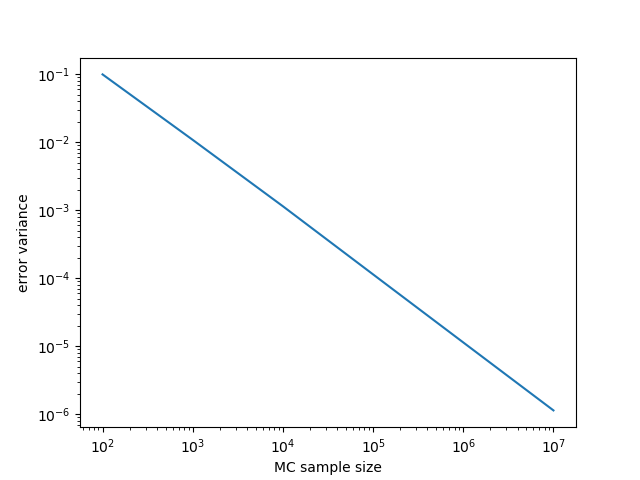
\includegraphics[width=.5\textwidth]{error_var.png}
      \caption{Error variance}
      \label{fig:error_var}
    \end{figure}
  \item
\end{enumerate}

\item
\begin{enumerate}[leftmargin=1em]
  \item
  \item
  \item
  \item
\end{enumerate}

\end{enumerate}

\end{document}